\section{Data}
\label{sec:data}

\subsection{Advertising spending}

I have collected data on government advertising spending (COMSOC), which includes the date (at the daily level) each contract was enforced, the name of the media outlet receiving funds, the name of the government agency contracting the media services or purchasing airtime, and the amount of money allocated. Importantly, I will be able to locate the media outlets that produce newspaper articles using the COMSOC data base as each media outlet that received money is classified into radio, online, newspapers, magazines, billboards, etc. 

During this period, the total amount of government advertising expenditure consistently exceeded the approved budgets, as illustrated in Figure \ref{fig:yearly_spending}. Each year, the Chamber of Deputies and the Senate must approve the budget allocated for advertising. Yet, throughout Peña Nieto's administration, actual spending regularly surpassed the authorized amounts by nearly double. This discrepancy not only raises suspicions but also underscores the underlying motives for such over-expenditure, suggesting a deliberate strategy to manipulate public perception and media content.

\begin{figure}[!htpb]
   \centering
   \caption{Evolution of the approved and exerted spending in government advertising spending}
   \label{fig:yearly_spending}
   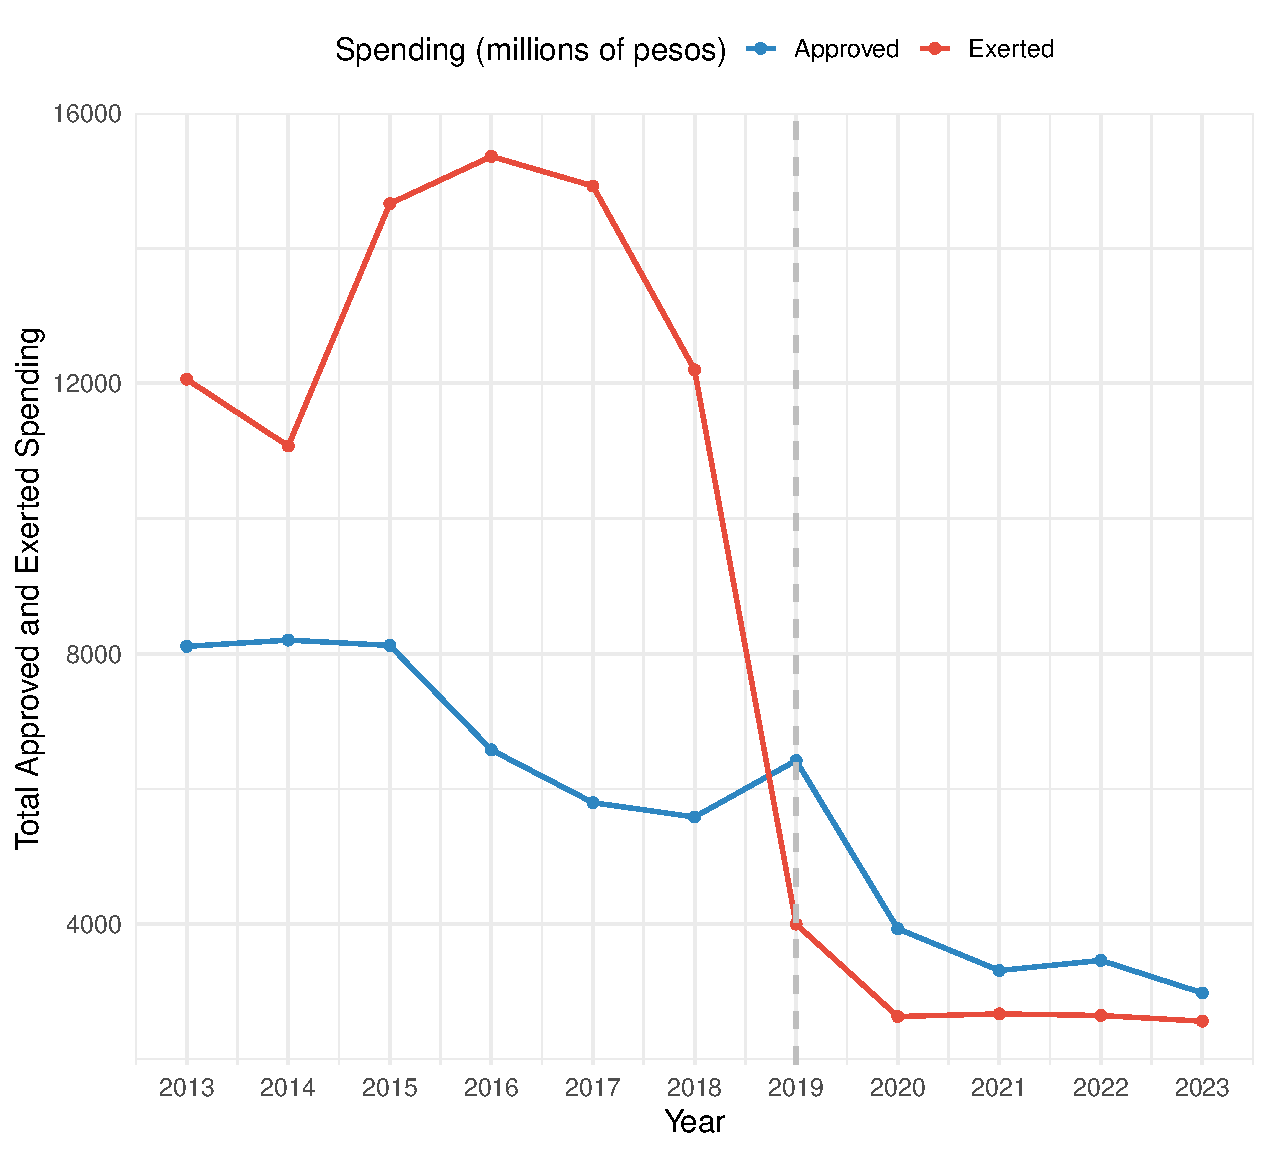
\includegraphics[width=.9\textwidth]{figures/descriptive_stats/ppto_article19.pdf}
   \caption*{ \footnotesize{\textit{Note:} This figure presents the yearly line trend (2012-2023) for the social advertising spending (on millions of pesos) from the Mexican government, divided by the spending approved by the Chamber of Deputies and the Senate at the beginning of that year (Blue) and the actual exerted spending (Red). The grey line represents the start of AMLO's tenure. Data was obtained from COMSOC and \citep{Article19}.}}
\end{figure}


\subsection{Newspaper data}

To compile a comprehensive dataset of newspaper articles that can be matched to this spending data, I will try to scrape a near-complete set of articles published online by newspapers from 2012 to 2024. I have started using web crawlers for data collection. At the moment I have fully scrapped the articles of 6 newspapers: La Jornada (top advertisement earner after the spending switch, left-leaning), Información Integral 24/7 (covers 5 states), AltaVoz (independent newspaper), Nexos (an opposition magazine, right-leaning) and Diario La Voz Oaxaca (local newspaper). Major media outlets like Reforma and Milenio have introduced paywalls on their websites, and some have complex HTML structures that make it difficult to extract articles directly. Therefore, for these more complex websites, I will prompt Google News Advanced Search daily for the relevant time period and for each media outlet. I'll use common Spanish words in each prompt to recover all the articles published that particular day and then collect each URL from the several result pages. 

Additionally, along with the news outlets that match the advertising spending database, I will aim to compile a set of independent newspapers to serve as a pure control group. To classify a media outlet as independent, I will use several criteria. The primary and most important criterion is that the outlet does not rely directly on government funding to operate. To assess this, I will first check if they appear in the advertising spending database for any year with available information. Second, I will visit each outlet’s website to review their disclosed funding sources. This process will also involve manual work to identify each media outlet’s official company name and founding date. For now I have identified a group of independent media outlets called \href{https://periodistasdeapie.org.mx/quienes-somos/}{Red de Periodistas de a Pie}, which is an NGO that consists of 14 media outlets located in different states in Mexico. None of them are in the COMSOC database, and as an NGO, their disclosed funding comes from international agencies and private companies.


Finally, to create the relevant outcome variables, I will categorize each post into one of three topics: economic, political, or crime/cartel-related violence. The primary focus of my analysis will be on violence-related articles, as my hypothesis suggests that this was the most salient issue at the time and the one the government sought to downplay. Thus, the main outcome variable will be the proportion of violence-related articles published by newspapers before and after the change in advertising spending.

Additionally, once I have identified posts related to economic and political topics, I will further analyze their tone and connotation. This will involve determining whether the articles are critical, positive, or negative and examining whether they report more or fewer corruption scandals compared to before the change in spending.

For the labeling process, I will proceed as follows. To the best of my knowledge, there is no available Spanish news dataset that explicitly labels each article as violence-related or not. Some efforts have been made to proxy cartel presence in specific municipalities during certain periods \citep{SobrinoCartel} and to approximate the number of violent acts, such as homicides, reported in the news \citep{Marshall}. The first approach used a web crawler to search Google News for cartel names (though not all violence in Mexico is cartel-related, nor do all articles about violence mention a cartel). The second approach relied on a simple word-matching method.

Given these limitations, and following recommendations for best replication practices in political science \citep{Spirling-Trust}, I will aim to create a training dataset using the labeled publications I have. I will then train a \href{https://github.com/dccuchile/beto}{BETO} model (BERT in Spanish), which is straightforward to replicate and has highly effective prediction capabilities.

For example, I have already scraped over 100,000 articles from La Jornada, which are labeled by categories such as political, economic, sports, opinion, etc. These can be used to train models for political and economic labels for newspapers that are not pre-labeled. For violence-related articles, I can apply the word-matching method from \citep{Marshall} to generate an initial random subset of positively identified articles related to violence, which I can then manually verify. This subset can serve as a basis for refining the model and distinguishing violence-related content from other categories, such as economic, sports, or opinion topics. If all else fails, I will employ an open-sourced LLM such as \href{https://www.llama.com/llama2/}{LLAMA 2}.